\documentclass[tikz, border=6pt]{standalone}
\usepackage[T1]{fontenc}
\usepackage{lmodern}
\usepackage{amsmath,amssymb,bm}
\usepackage{lmodern}
\usetikzlibrary{arrows.meta}
\definecolor{Blue}{HTML}{3A76D8}
\definecolor{Yellow}{HTML}{EAB531}
\definecolor{Orange}{HTML}{EE8133}
\definecolor{Purple}{HTML}{8459D1}
\definecolor{Ink}{HTML}{1F2937}
\begin{document}
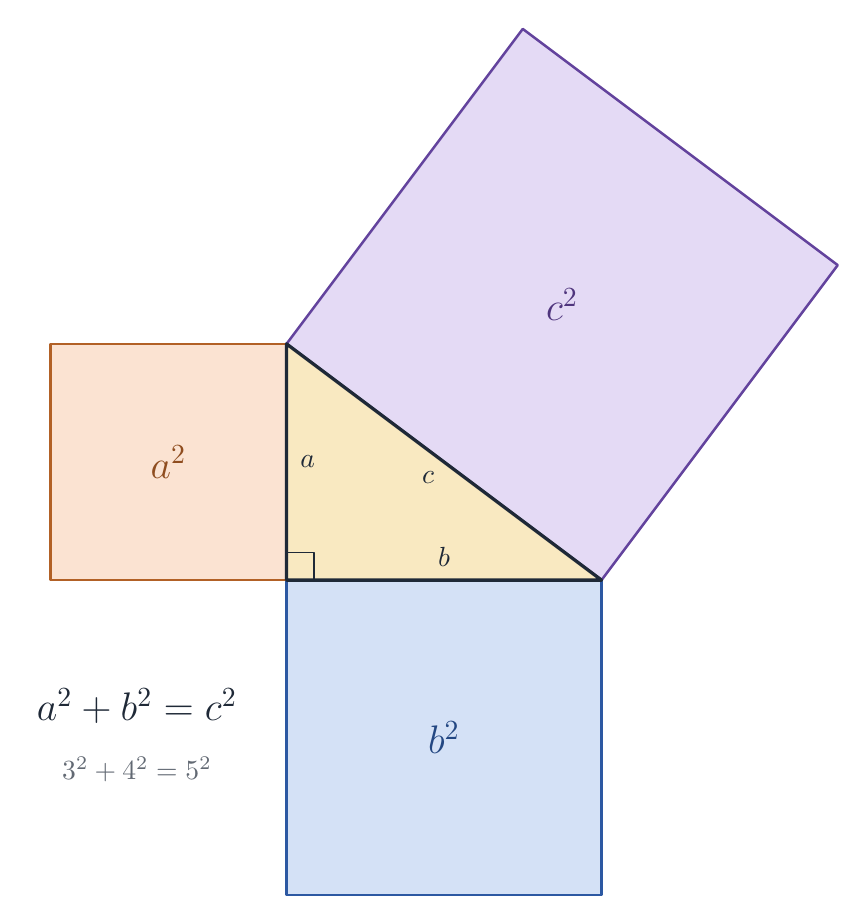
\begin{tikzpicture}[color=Ink, line width=0.5pt, >={Latex[length=5pt, width=3.6pt]}, line join=round]
  \draw[fill=Blue!22, draw=Blue!75!black, line width=0.9pt] (0,0) -- (4,0) -- (4,-4) -- (0,-4) --
      cycle;
  \node[font=\Large, text=Blue!60!black] at (2,-2) {$b^2$};
  \draw[fill=Orange!22, draw=Orange!75!black, line width=0.9pt] (0,3) -- (0,0) -- (-3,0) -- (-3,3) --
      cycle;
  \node[font=\Large, text=Orange!60!black] at (-1.5,1.5) {$a^2$};
  \draw[fill=Purple!22, draw=Purple!75!black, line width=0.9pt] (4,0) -- (0,3) -- (3,7) -- (7,4) --
      cycle;
  \node[font=\Large, text=Purple!60!black] at (3.5,3.5) {$c^2$};
  \draw[fill=Yellow!30, line width=1.2pt] (0,0) -- (4,0) -- (0,3) -- cycle;
  \draw (0.35,0) -- (0.35,0.35) -- (0,0.35);
  \node[anchor=south, yshift=0.05cm] at (2,0) {$b$};
  \node[anchor=west, xshift=0.05cm] at (0,1.5) {$a$};
  \node[anchor=north east] at (2,1.5) {$c$};
  \node[font=\Large] at (-1.9,-1.6) {$a^2 + b^2 = c^2$};
  \node[font=\normalsize, text=Ink!70] at (-1.9,-2.4) {$3^2 + 4^2 = 5^2$};
\end{tikzpicture}
\end{document}
